\section{Ring Loading Problems and Complexity}

Definition of (Integer) Ring Loading also as decision problem

Definition of Relaxed Ring Loading also as decision problem

Complexity of Ring Loading and Relaxed Ring Loading

Interval-notation for ring interpreted as equivalence classes of finite ring.

\begin{notation}
	Let $1 \leq i < j \leq n$.
	Then we write $[i, j) \coloneqq \{i, i+1, \ldots, j-2, j-1\}$.
	We also define $[j, i) \coloneqq \{j, j+1, \ldots, n-1, n, 1, \ldots, i-2, i-1\}$.
	Open, half-open and closed intervals are to be interpreted in the same manner as real intervals.
\end{notation}

\begin{problem}{Ring Loading}
	\textbf{In:} Ring of size $n \in \N$, demands $d_{ij} \in \R^+$ for $1 \leq i < j \leq n$.\\
	\textbf{Goal:} Find a function $\Phi: \{(i, j)~|~1 \leq i < j \leq n\} \rightarrow \{0, 1\}$ such that
	$\max_{1 \leq i \leq n} L_i$ is minimal, where
	\begin{equation}
		L_i(\phi) \coloneqq \ldots
	\end{equation}
\end{problem}
Ring loading is a routing problem where traffic must be routed either through the front or the back.

The cases $n = 1, 2$ are trivial and $n = 3$ has a solution independent of demands (see figure XX). Hence we assume $n \geq 4$ at all times.

$\phi(i, j) = 1$ means that the traffic from the demand $d_{ij}$ is routed through the path $\{i, i+1, \ldots, j-1, j\}$.
This route is called the \emph{front route}.
Otherwise, if $\phi(i, j) = 0$, the traffic is routed through $\{j, j+1, \ldots, n-1, n, 1, \ldots, i\}$, which is called the \emph{back route}.
The back route always contains the link $\{n, 1\}$.

\begin{theorem}
	The decision form of \RL is NP-complete.
\end{theorem}
\begin{proof}
	\Todo{Input can be encoded in O(n**2) space}
	A function $\Phi$ of the desired form can be encoded using $\cO(n^2)$ space, e.g. as a binary array, and serves as witness for \RL.
	This implies that \RL is in NP.
	In order to show NP-completeness, we provide a polynomial-reduction of the \textsc{Partition} problem \cite{karp72}.
	This problem asks whether, given $m$ integers $\{z_1, \ldots, z_m\}$, there exists an $S \subseteq [m]$ such that 
	\begin{equation}
		\sum_{i \in S} z_i = \sum_{j \in [m] \setminus S} z_j \ .
	\end{equation}
	
\end{proof}

\begin{definition}
	Let $1 \leq g < h \leq n$.
	A \emph{cut} $\{g, h\}$ is a set of two links $\{\{g, g+1\}, \{h, h+1\}\}$.
	A demand $d_{ij}$ is said to \emph{cross} a cut $\{g, h\}$ if exactly one of $i$ and $j$ lies within $[g, h)$.
	The \emph{total demand across $\{g, h\}$} is defined as
	\begin{equation}
		D_{gh} \coloneqq \sum_{\{d_{ij}~|~d_{ij}\ \text{crosses}\ \{g, h\}\}} d_{ij} \ .
	\end{equation}
	This is the sum of the demands that must cross either $\{g, g+1\}$ or $\{h, h+1\}$.
\end{definition}

\begin{figure}
	\centering
	\begin{minipage}[t]{.5\textwidth}
		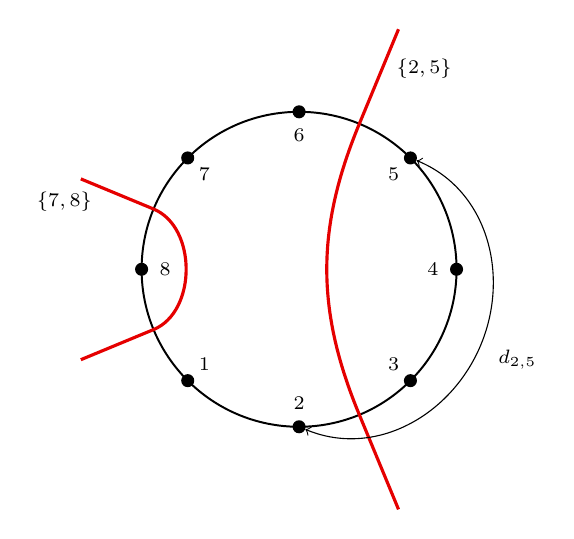
\begin{tikzpicture}[font=\scriptsize, node/.style={circle,thick,draw},
		l_2/.style={line width =0.25mm},
		scale=1, transform shape]
			% equidistant points and arc
			\foreach \x [count=\p] in {0,...,7} {
				\node[shape=circle,fill=black, scale=0.5] (\p) at (\x*45-135:2) {};
			};
			\foreach \x [count=\p] in {0,...,7} {
				\draw (225 + \x*45:1.7) node {\p};
%				\draw (-30-\x*60:2.4) node {$\bar{\p}$};
			}; 
			\draw[l_2] (4) arc (0:360:2);
			
			\draw[line width=0.4mm, red!90!black] (67.5:3.3) to [out=-112.5,in=67.5] (67.5:2) to [out=-112.5,in=112.5] (-67.5:2) to [out=-67.5, in=112.5](-67.5:3.3);
			\node (cut1) at (58:3) {$\{2, 5\}$};
			
			\draw[line width=0.4mm, red!90!black] (157.5:3) to [out=-22.5,in=157.5] (157.5:2) to [out=-22.5,in=22.5] (-157.5:2) to [out=-157.5, in=22.5](-157.5:3);
			\node (cut2) at (164:3.1) {$\{7, 8\}$};
			
			\node (a) at (-22.5:3) {$d_{2, 5}$};
			\draw[<->] (2)  to [out=-22.5,in=-112.5] (-22.5:2.5) to [out=67.5,in=-22.5](5);
%			\node (b) at (-67.5:2.8) {$d_{1, 4}$};
%			\draw[<->] (1)  to [out=-67.5,in=-157.5] (-67.5:2.5) to [out=22.5,in=-67.5] (4);
			
			\node (bottom) at (0, -2.8) {};
			%		\draw[dashed] (1) -- (3) -- (5) -- (1);
			% axes
			%		\draw [dotted, gray] (-2.6,0) -- (2.6,0);
			%		\draw [dotted, gray] (0,-2.15) -- (0,2.15);
		\end{tikzpicture}
	\end{minipage}
	\caption{Examples of cuts (red).
	We imagine a cut as a chord connecting the midpoints of its edges.
	The demand $d_{2, 5}$ crosses the cut $\{2, 5\}$ and is parallel to the cut $\{7, 8\}$.
	The cuts $\{2, 5\}$ and $\{7, 8\}$ are parallel.}
	\label{fig:cut-example}
\end{figure}

We can formulate a relaxed version of \RL, which allows demands to be routed both ways around the ring.
\begin{problem}{Relaxed Ring Loading}
	\textbf{In:} Ring of size $n \in \N$, demands $d_{ij} \in \R^+$ for $1 \leq i < j \leq n$.\\
	\textbf{Goal:} Find a function $\phi: \{(i, j)~|~1 \leq i < j \leq n\} \rightarrow [0, 1]$ such that $\max_{1 \leq i \leq n} L_i^\ast$ is minimal, where
	\begin{equation}
		L_i^\ast(\phi) \coloneqq \ldots
	\end{equation}
\end{problem}
In contrast to its binary version, \RRL can be solved in polynomial time, as it can be formulated as the following linear problem
\begin{alignat}{2}
	&\min &\quad& L\\
	&s.t. &\quad& L \geq L_i^\ast(\Phi)\quad \forall 1 \leq i \leq n \ .
\end{alignat}
Note that the $L_i$ are linear functions.
